\documentclass[11pt]{article}

\usepackage[margin=1in]{geometry}
\usepackage{booktabs}
\usepackage{float}
\usepackage{graphicx}
\usepackage[hidelinks]{hyperref}

\graphicspath{{../outputs/figures/}}
\setlength{\parindent}{0pt}
\setlength{\parskip}{0.6em}

\title{Interpretation of Random Forest Partial Dependence Plots}
\author{
    Adriá Aguilar Mínguez, Pablo Gandía Miñana, Santiago Font Piña \\
    \small  ALT
}
\date{\today}

\begin{document}
\maketitle

\section{Summary}

This report explains two random forest regression models using Partial Dependence Plots (PDPs). The first model predicts daily bike rentals from calendar and normalized weather data. The second model predicts King County house prices from a focused set of property characteristics.

For bike rentals, the model indicates that demand increases strongly over the two-year period and is highest at moderate-to-warm normalized temperatures. High humidity and high windspeed reduce expected rentals. The two-dimensional PDP shows that the best weather profile for demand is warm and not highly humid, while cold and humid conditions are the weakest demand environment.

For house prices, living area is the dominant driver among the selected features. Bathrooms also show a positive relationship with predicted price. Bedrooms have a much weaker marginal effect after controlling for living area and the other selected variables, which is useful for valuation decisions because it suggests that usable space matters more than room count alone.

\section{Methodology}

A PDP estimates the marginal relationship between one or two input features and the model prediction. For a selected feature value, the method replaces that feature in a reference sample, predicts all modified observations with the trained model, and averages the predictions. PDPs explain the behavior of the fitted model, not a causal effect in the real world.

Sampling is used for PDP calculation because the method requires repeated prediction over many modified datasets. This keeps computation manageable while preserving a representative set of background records for averaging. The analysis uses a fixed random seed of 2024.

\begin{table}[H]
\centering
\caption{Model configuration and out-of-bag performance}
\begin{tabular}{lrrrrr}
\toprule
Dataset & Training rows & PDP rows & Trees & OOB RMSE & OOB $R^2$ \\
\midrule
Daily bike rentals & 731 & 50 & 500 & 636.0 & 0.892 \\
King County house prices & 1500 & 1500 & 500 & 218845.5 & 0.600 \\
\bottomrule
\end{tabular}
\end{table}

The bike rental model uses all available daily records for training and 50 sampled observations for PDP calculation. The target is \texttt{cnt}. The weather axes in the bike PDPs use the original normalized dataset scales: \texttt{temp}, \texttt{hum}, and \texttt{windspeed}. 

The house price model uses 1500 sampled complete observations for both model training and PDP calculation. The target is \texttt{price}. The selected predictors are \texttt{bedrooms}, \texttt{bathrooms}, \texttt{sqft\_living}, \texttt{sqft\_lot}, \texttt{floors}, and \texttt{yr\_built}.

\section{Bike Rental Demand}

\subsection{One-Dimensional PDP Results}

\begin{figure}[H]
\centering
\begin{tabular}{cc}
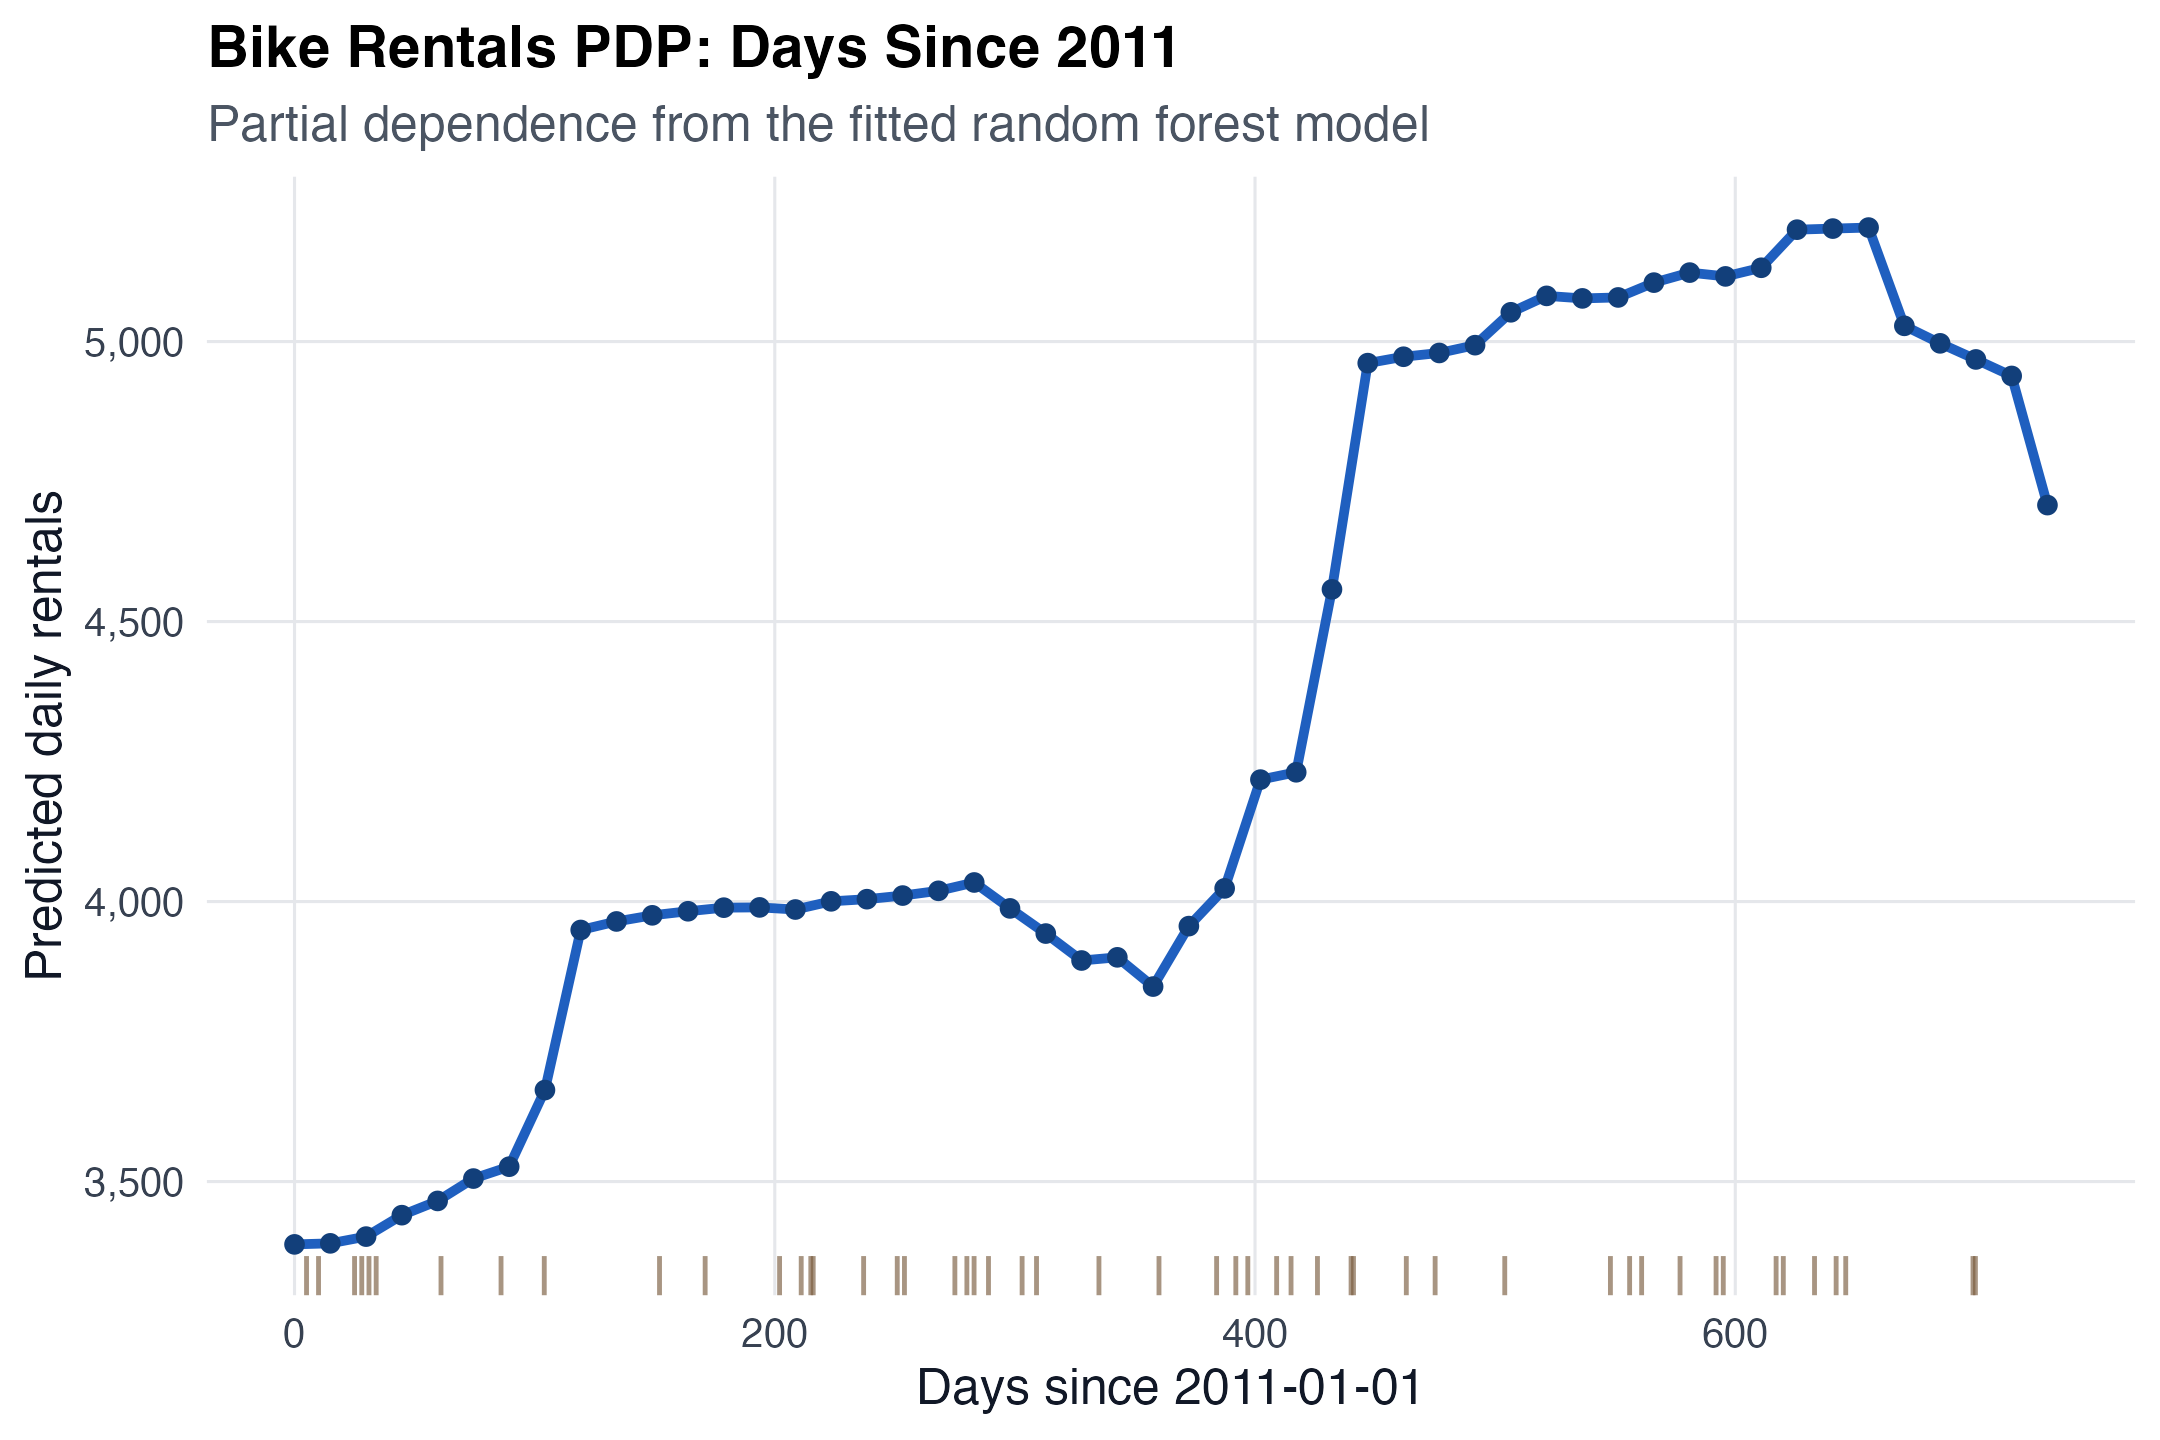
\includegraphics[width=0.46\textwidth]{bike_pdp_days_since_2011.png} &
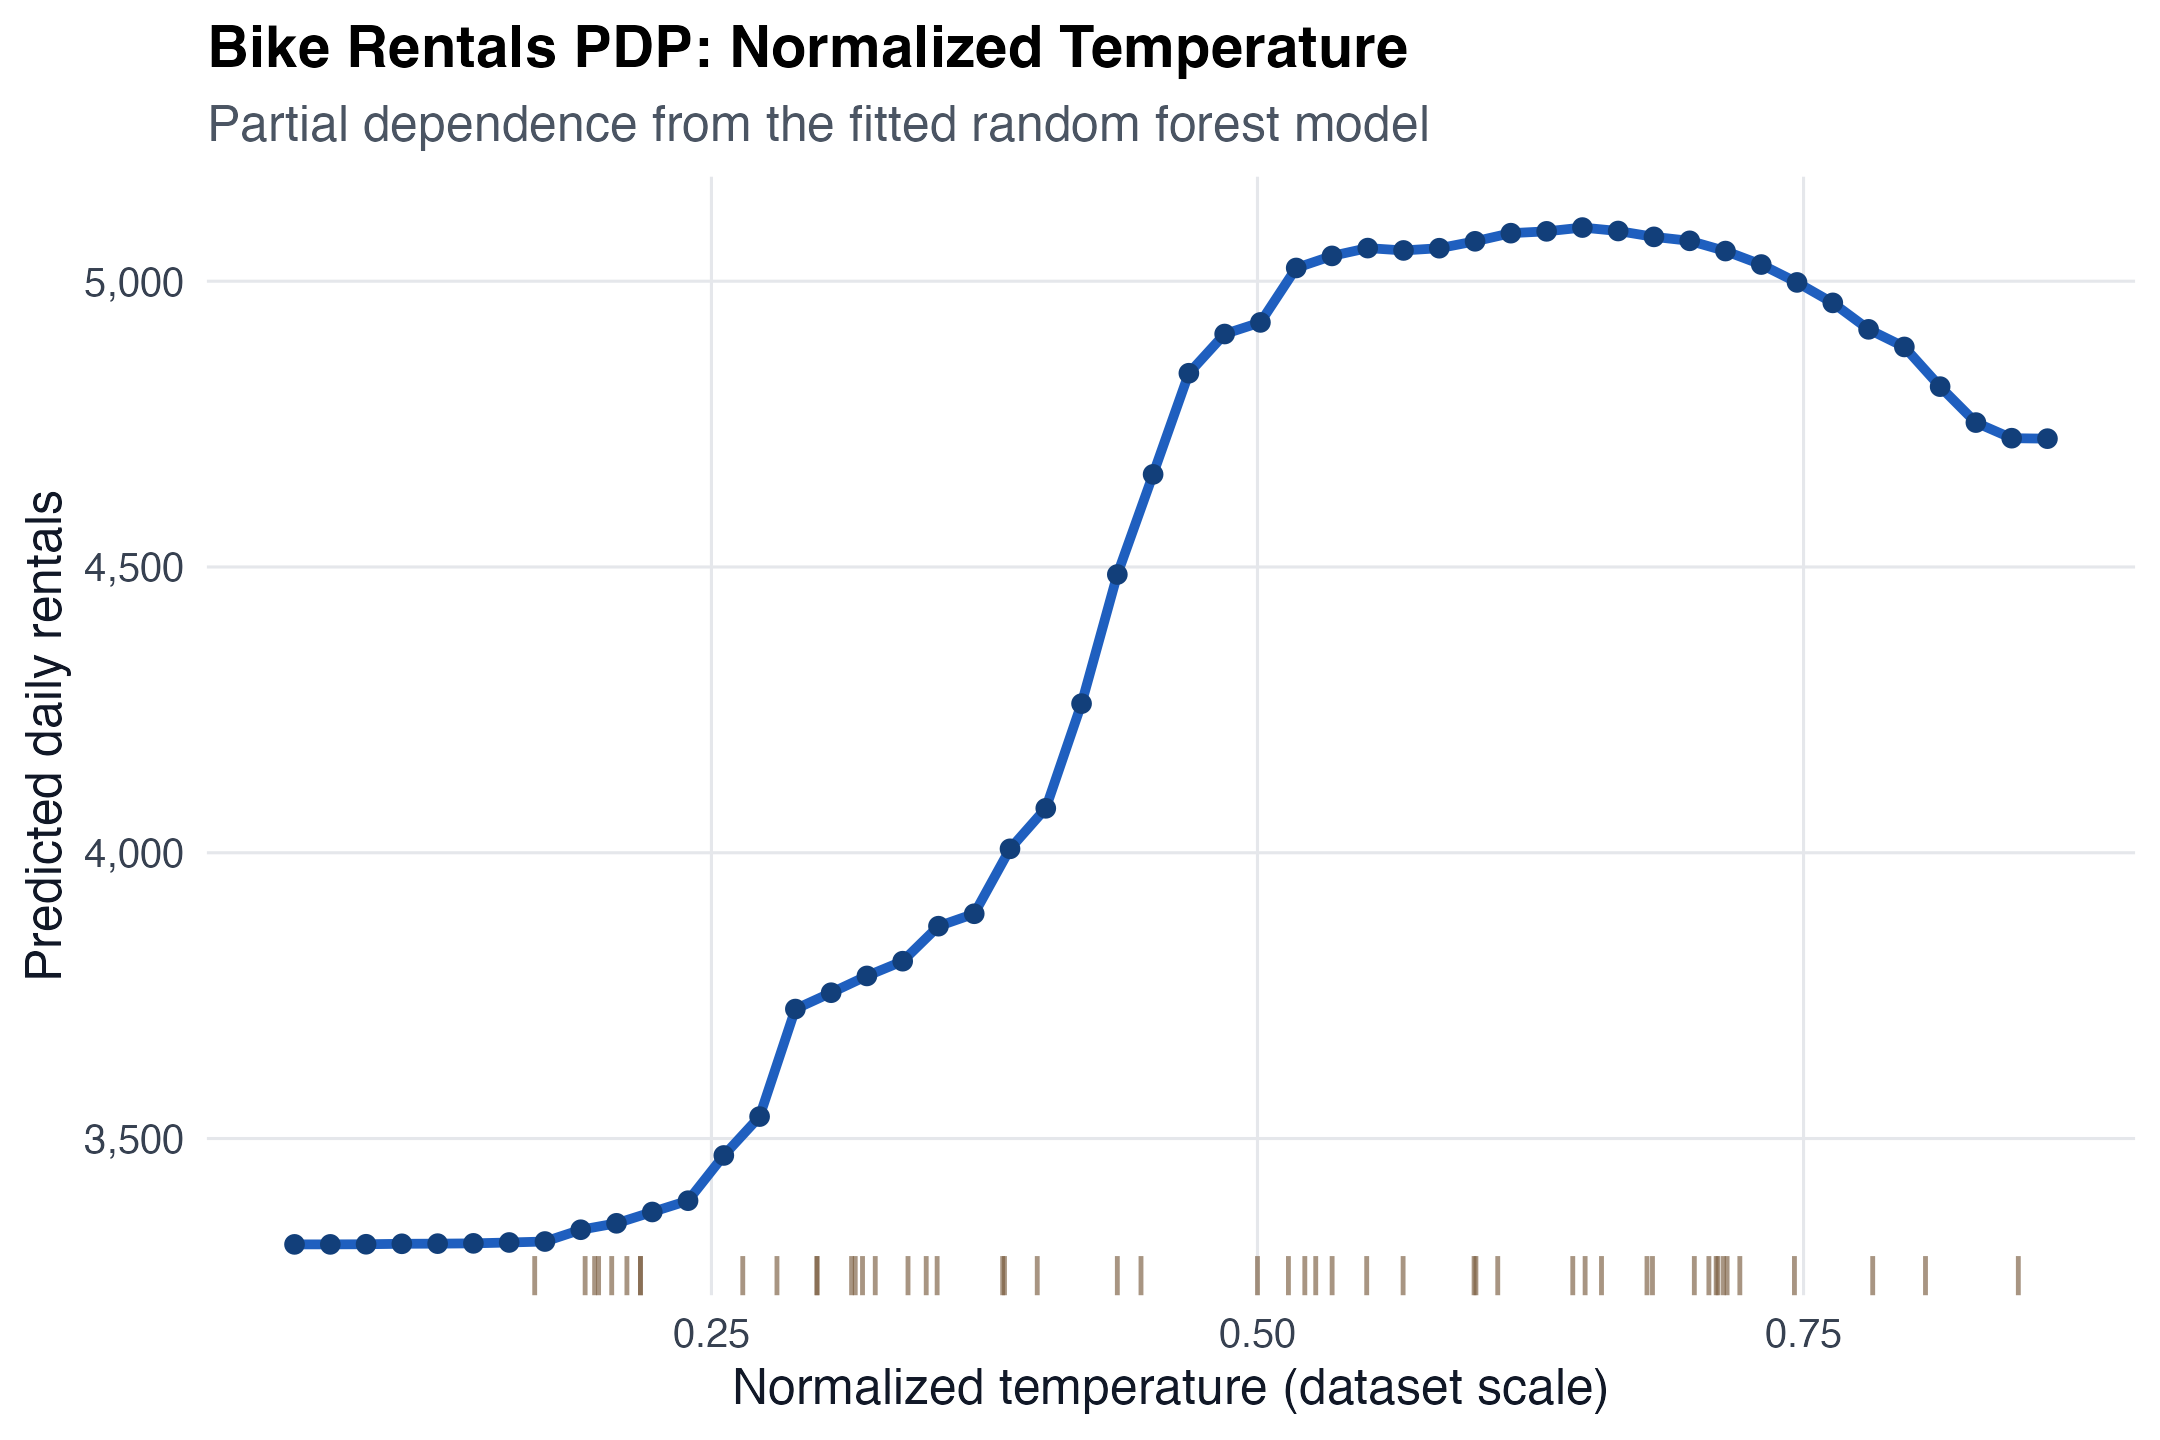
\includegraphics[width=0.46\textwidth]{bike_pdp_temperature.png} \\
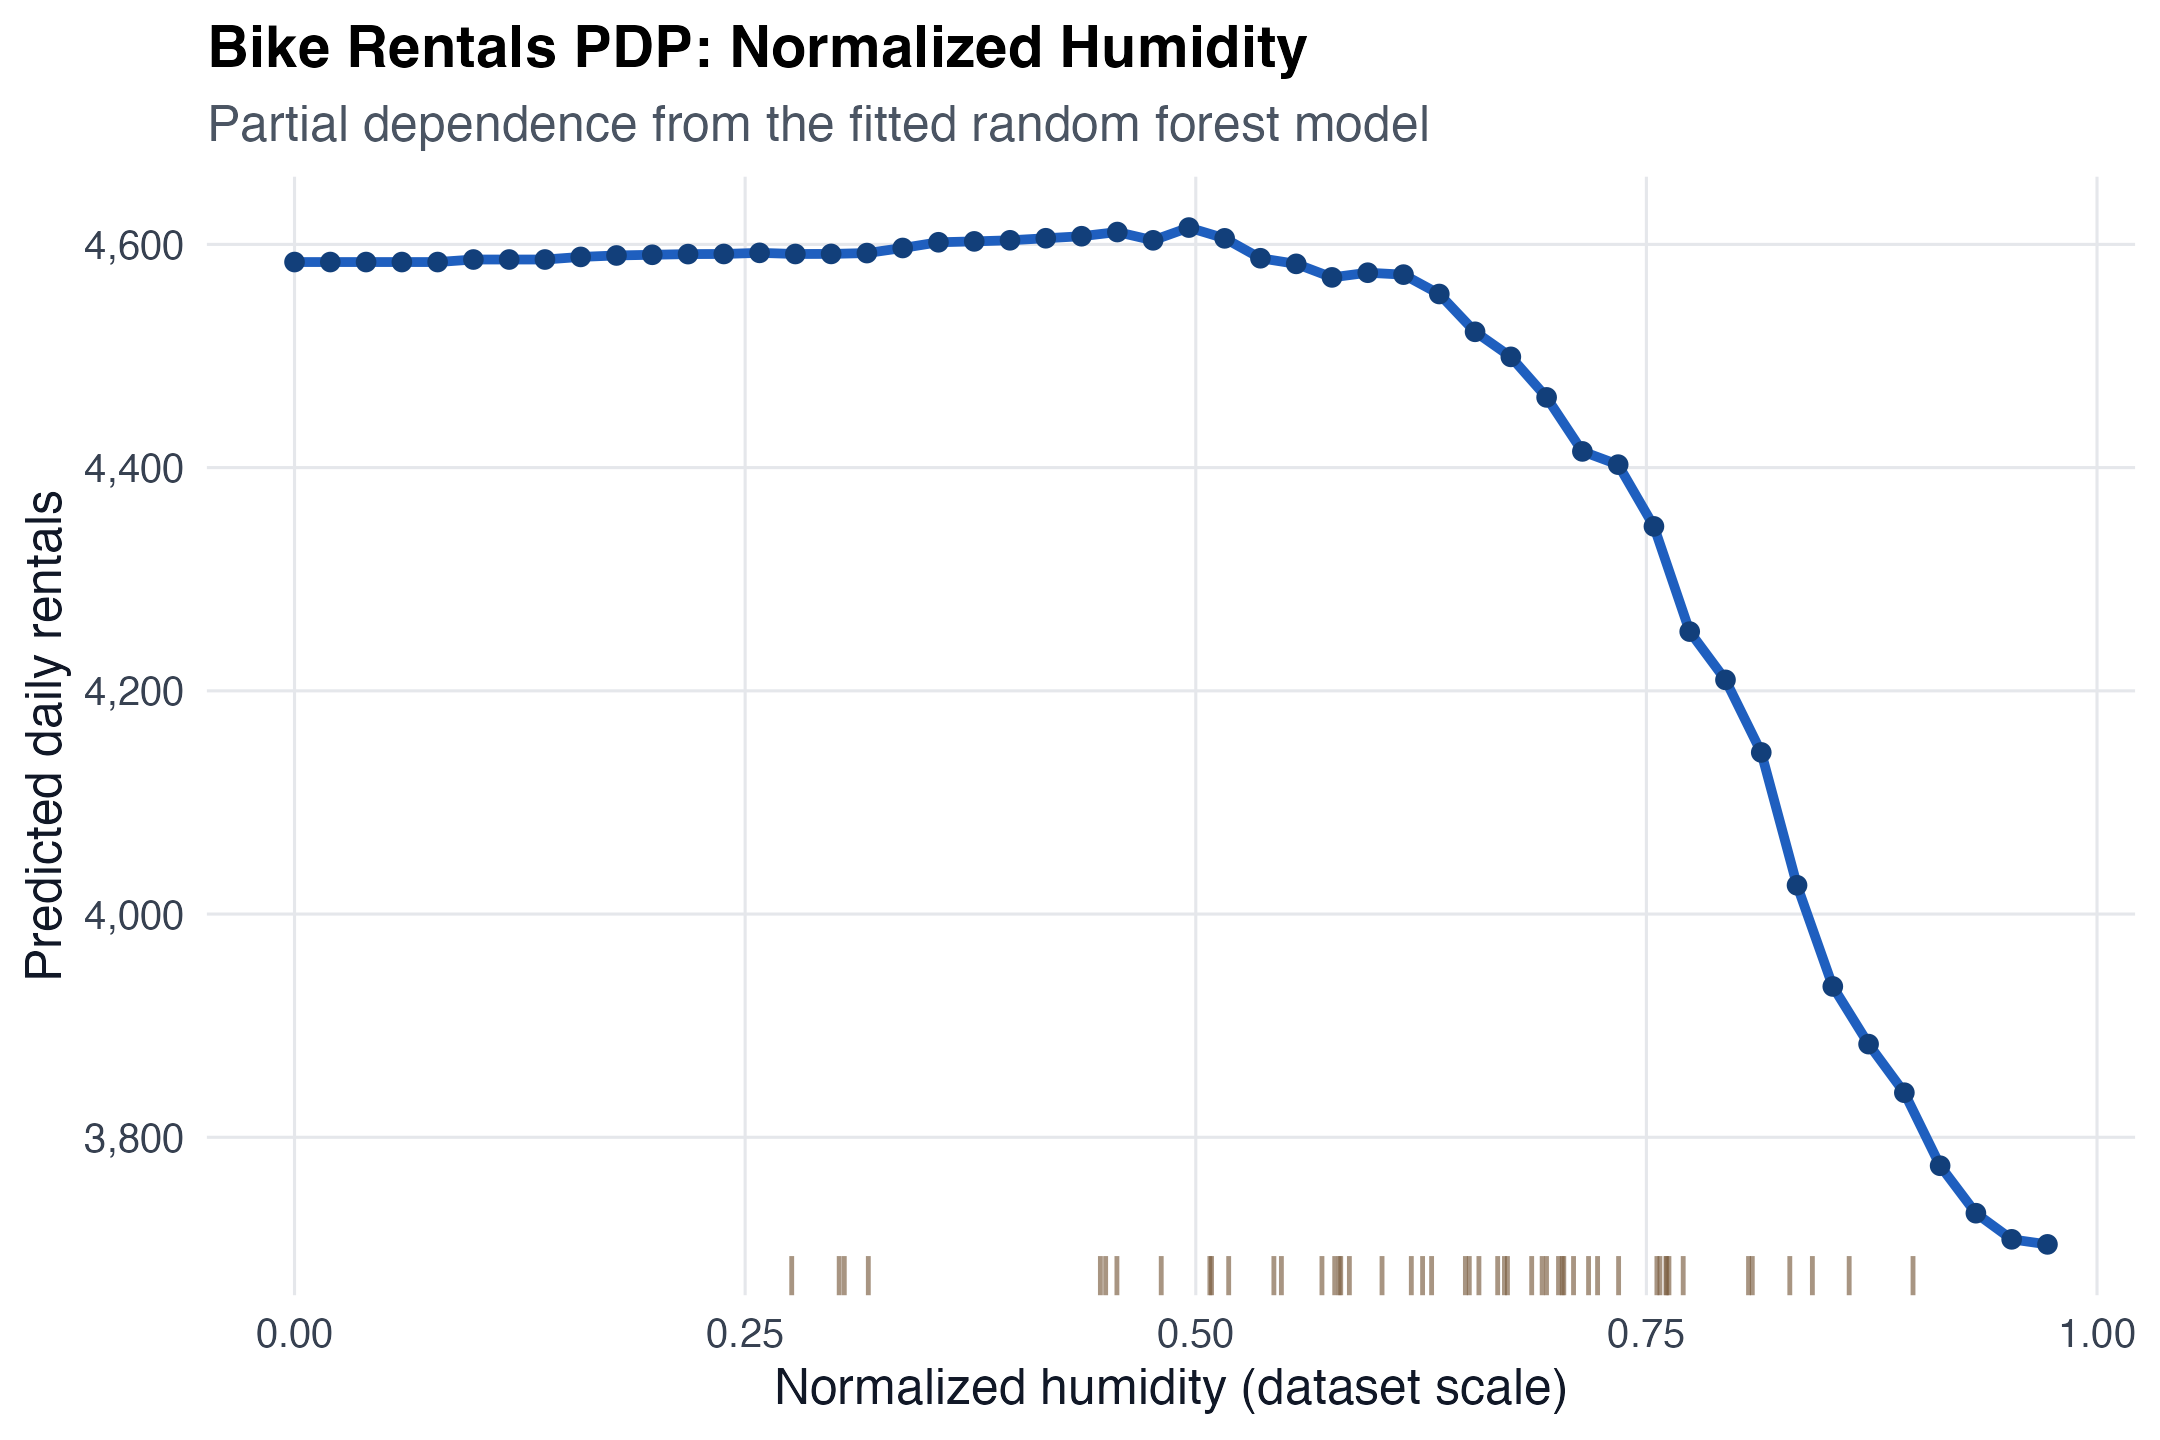
\includegraphics[width=0.46\textwidth]{bike_pdp_humidity.png} &
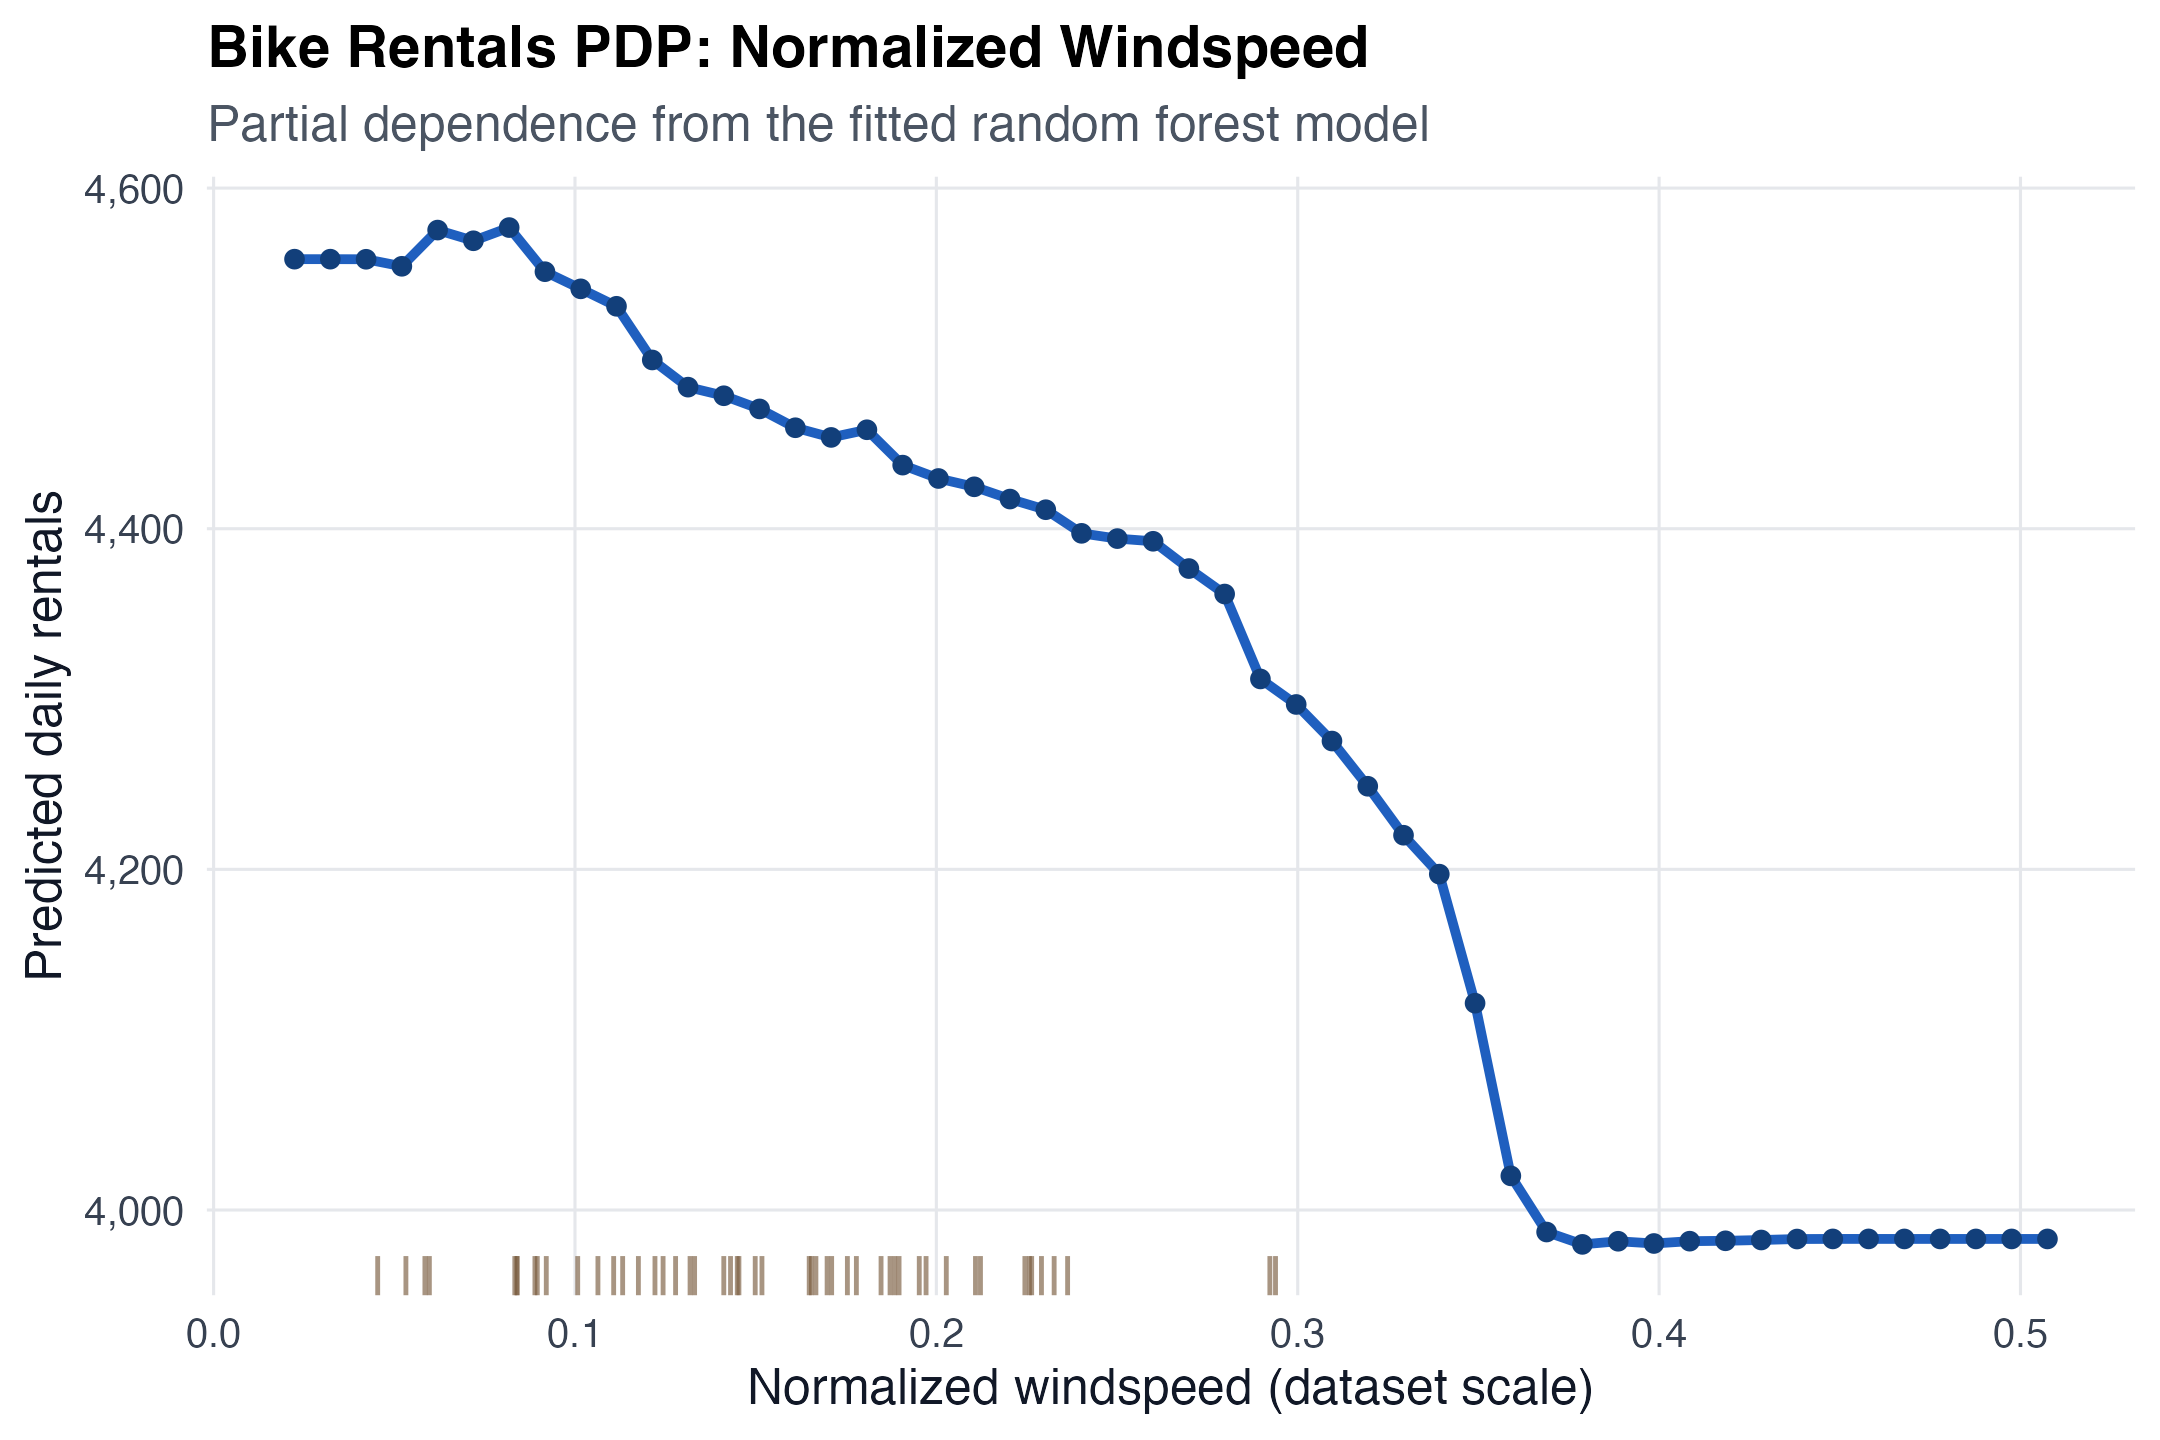
\includegraphics[width=0.46\textwidth]{bike_pdp_windspeed.png}
\end{tabular}
\caption{One-dimensional PDPs for daily bike rental demand.}
\end{figure}

\textbf{Days since 2011.}
The model predicts materially higher daily rental volume later in the period. Predicted demand rises from roughly 3,400 rentals at the start of the series to more than 5,200 at the high end of the PDP. For a bike rental operator, this suggests a strong structural growth pattern across the observed period. Capacity planning, maintenance staffing, and inventory allocation should therefore account for a rising baseline demand level rather than relying only on weather conditions.

\textbf{Temperature.}
Temperature is one of the strongest weather drivers in the model. Predicted rentals increase sharply as temperature moves from cold values toward the higher range. Above that range, the PDP flattens and then declines slightly. Operationally, moderate-to-warm days should be treated as high-demand days, while the hottest normalized values do not continue to add demand at the same rate.

\textbf{Humidity.}
Humidity has a negative business signal at higher values. The PDP is comparatively stable through moderate humidity, but predicted rentals fall as humidity approaches the upper range. This suggests that very humid days should be planned with more conservative rental expectations, even if temperature is otherwise favorable.

\textbf{Wind speed.}
The windspeed PDP shows lower predicted rentals at higher windspeed values. The effect is smaller than temperature but still operationally relevant. Windy days can reduce casual usage and should be considered in short-term demand forecasts.

\subsection{Two-Dimensional PDP Result}

\begin{figure}[H]
\centering
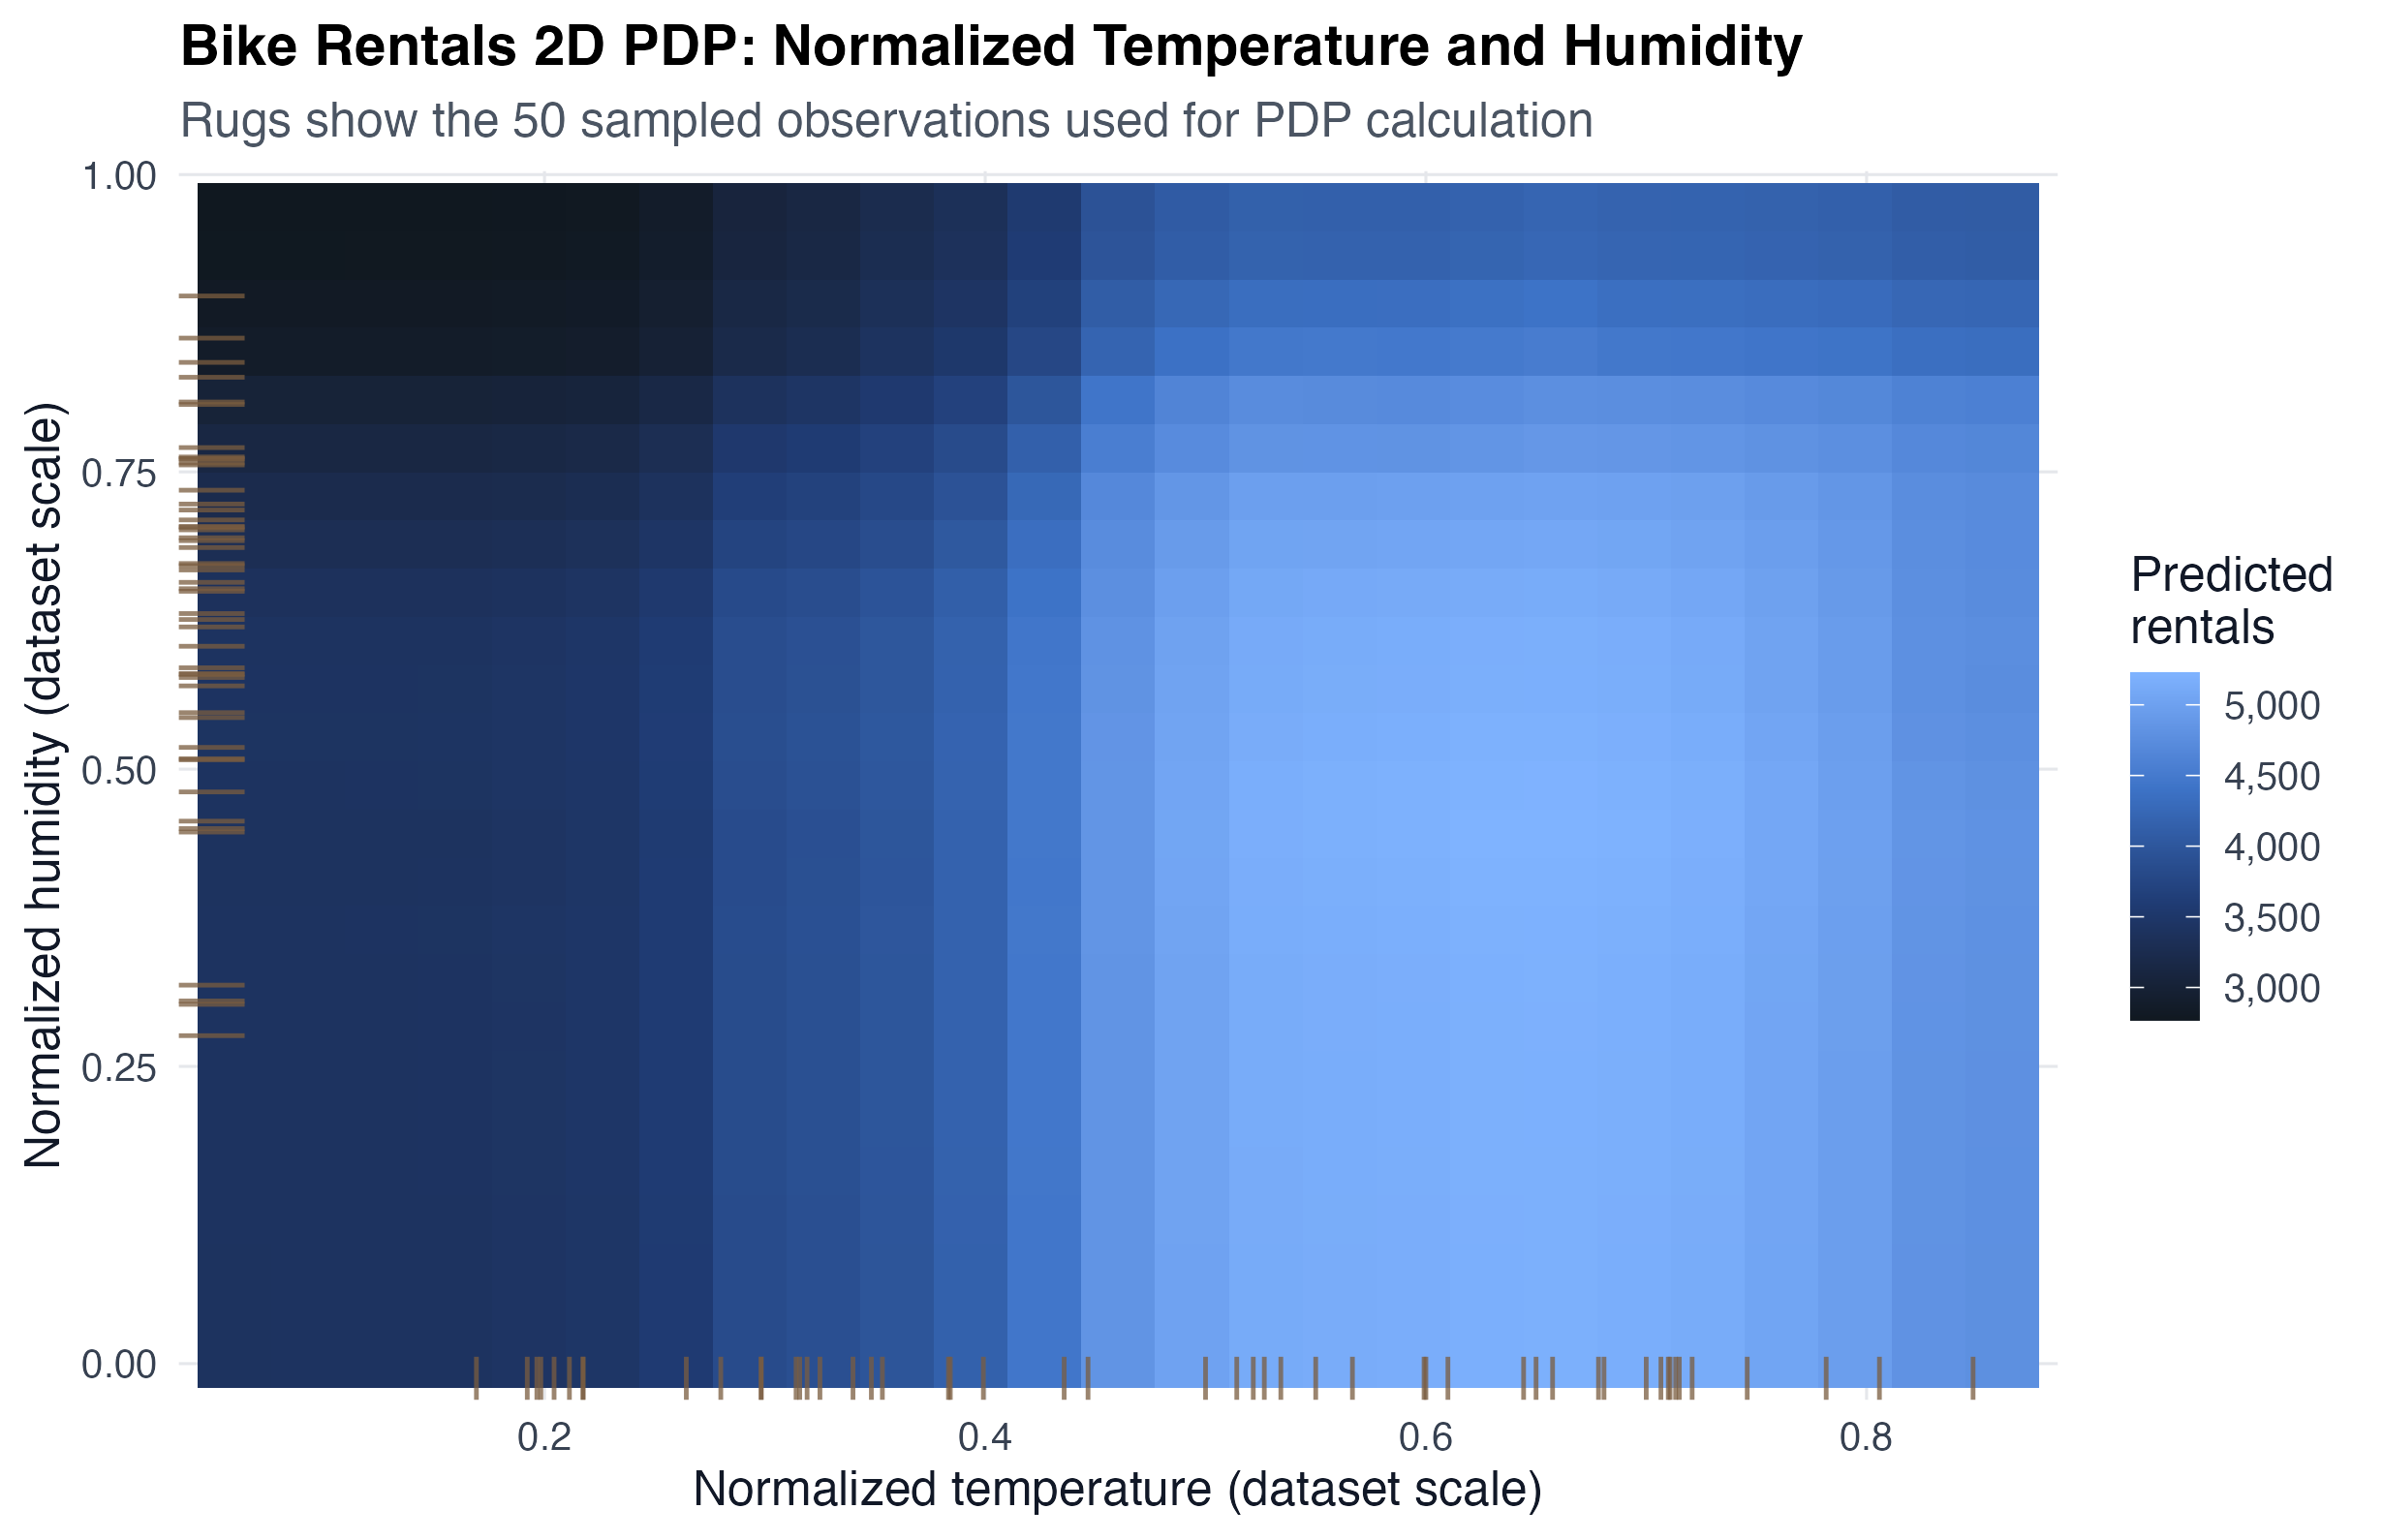
\includegraphics[width=0.92\textwidth]{bike_pdp_2d_temperature_humidity_heatmap.png}
\caption{Two-dimensional PDP for temperature and humidity.}
\end{figure}

The two-dimensional PDP confirms that temperature and humidity should be interpreted together. The highest predicted rentals occur at warmer normalized temperatures with low-to-moderate humidity. Cold and humid combinations are the weakest region. The heatmap therefore supports weather-aware planning: favorable temperature alone is not enough if humidity is very high.

\section{House Price Drivers}

\subsection{One-Dimensional PDP Results}

\begin{figure}[H]
\centering
\begin{tabular}{cc}
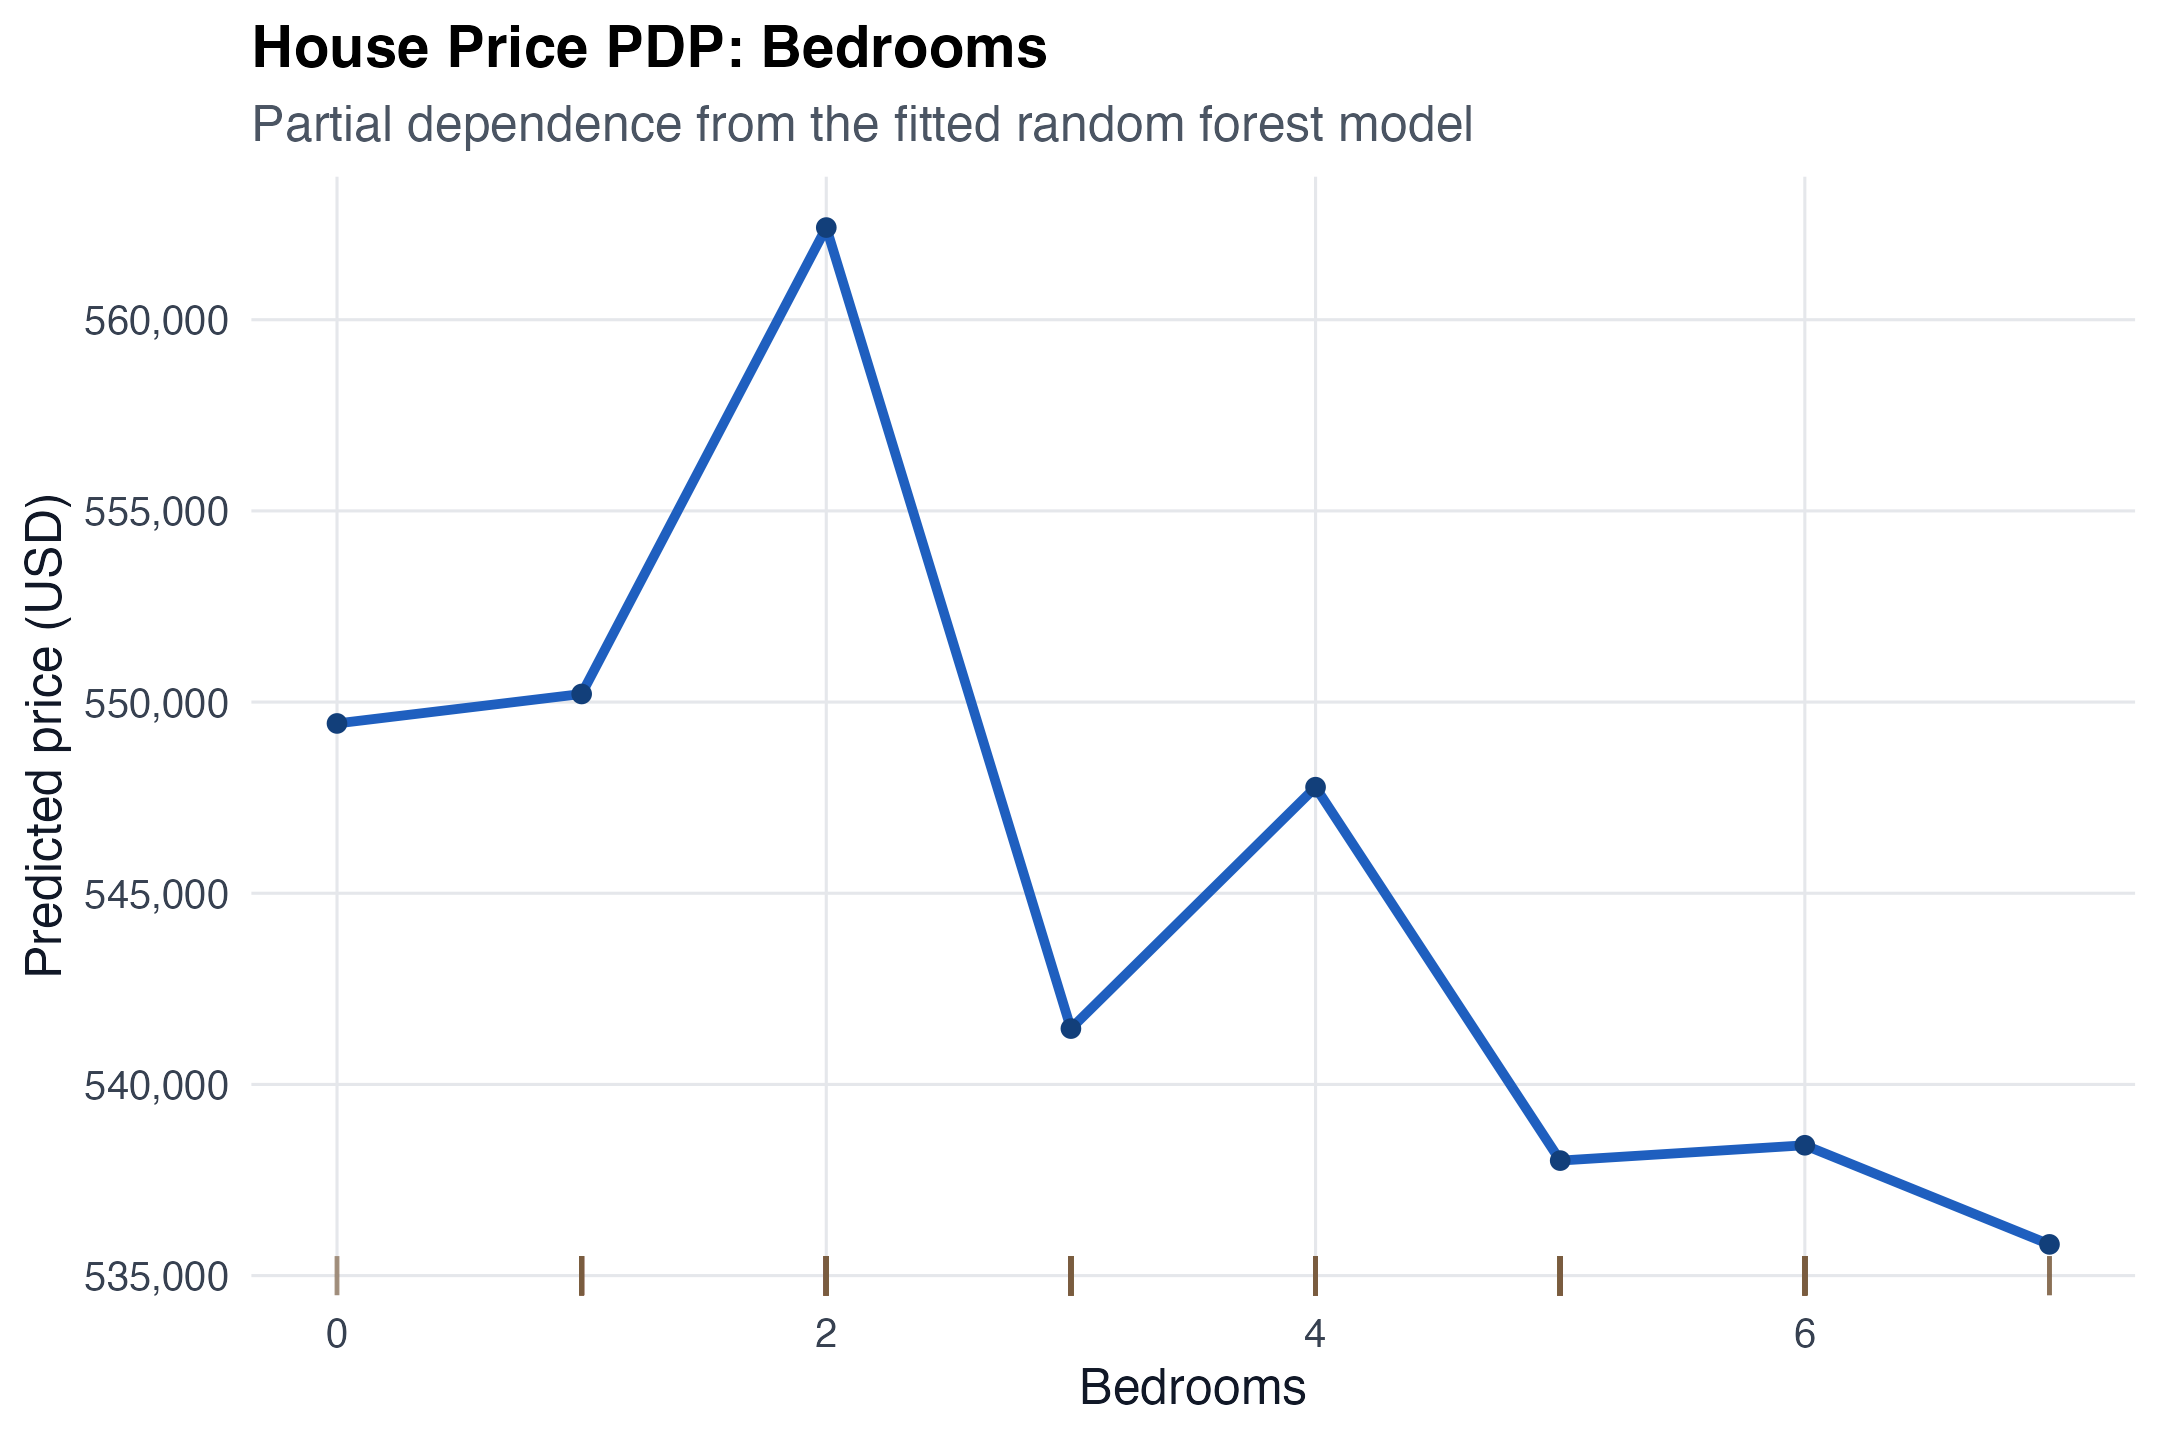
\includegraphics[width=0.46\textwidth]{house_pdp_bedrooms.png} &
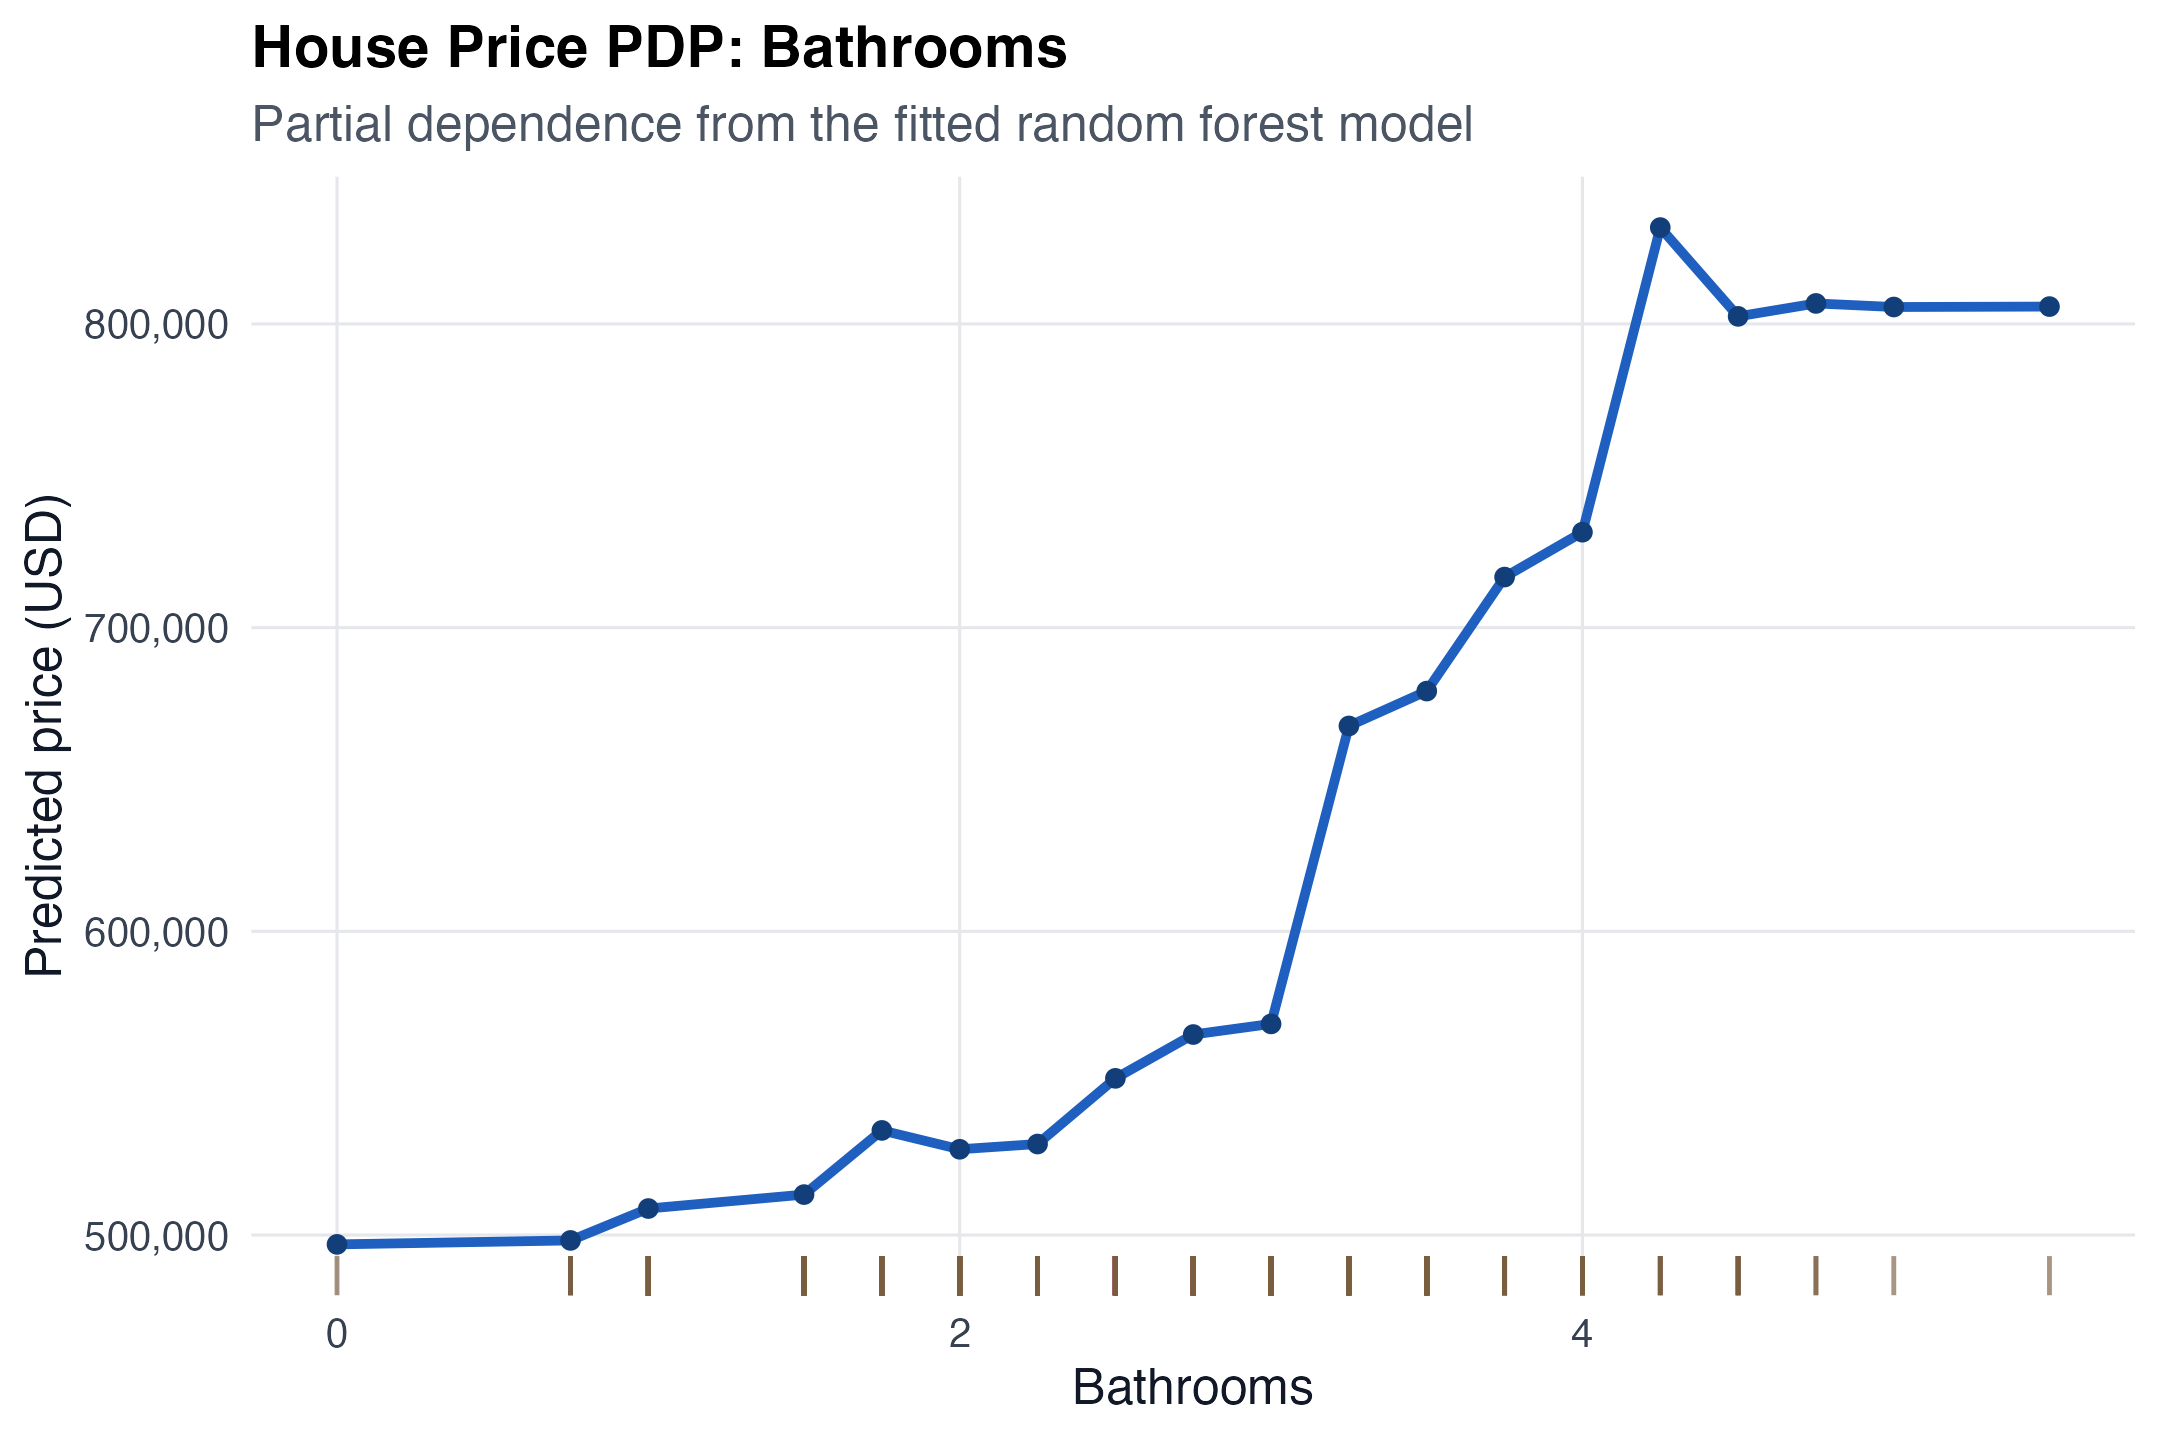
\includegraphics[width=0.46\textwidth]{house_pdp_bathrooms.png} \\
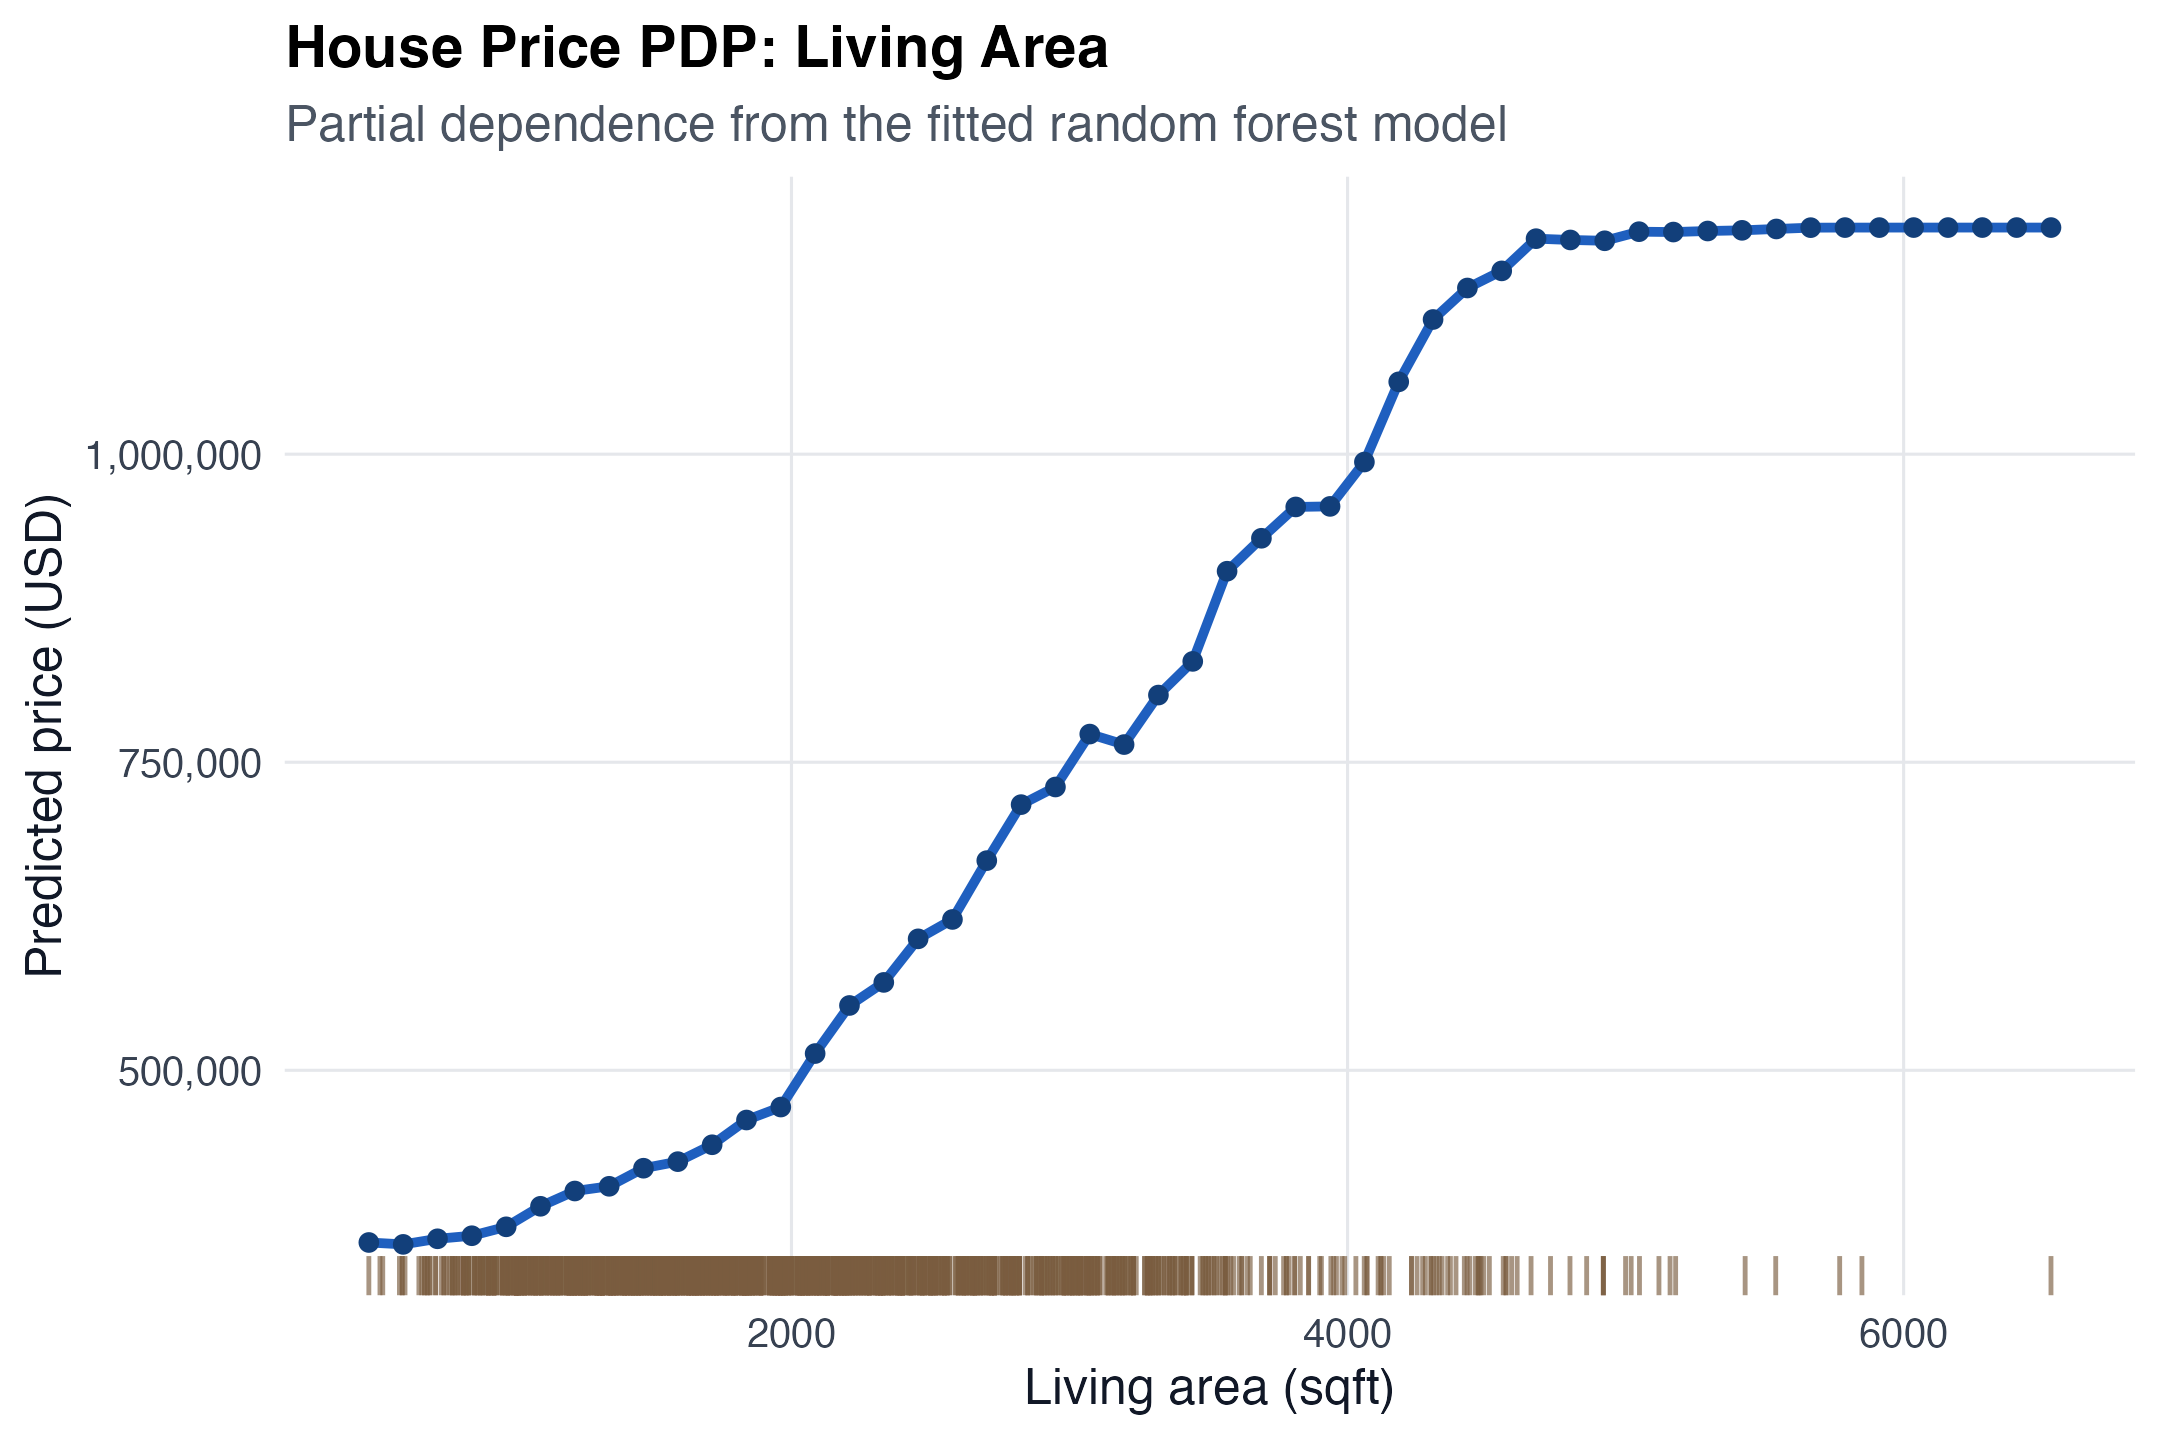
\includegraphics[width=0.46\textwidth]{house_pdp_sqft_living.png} &
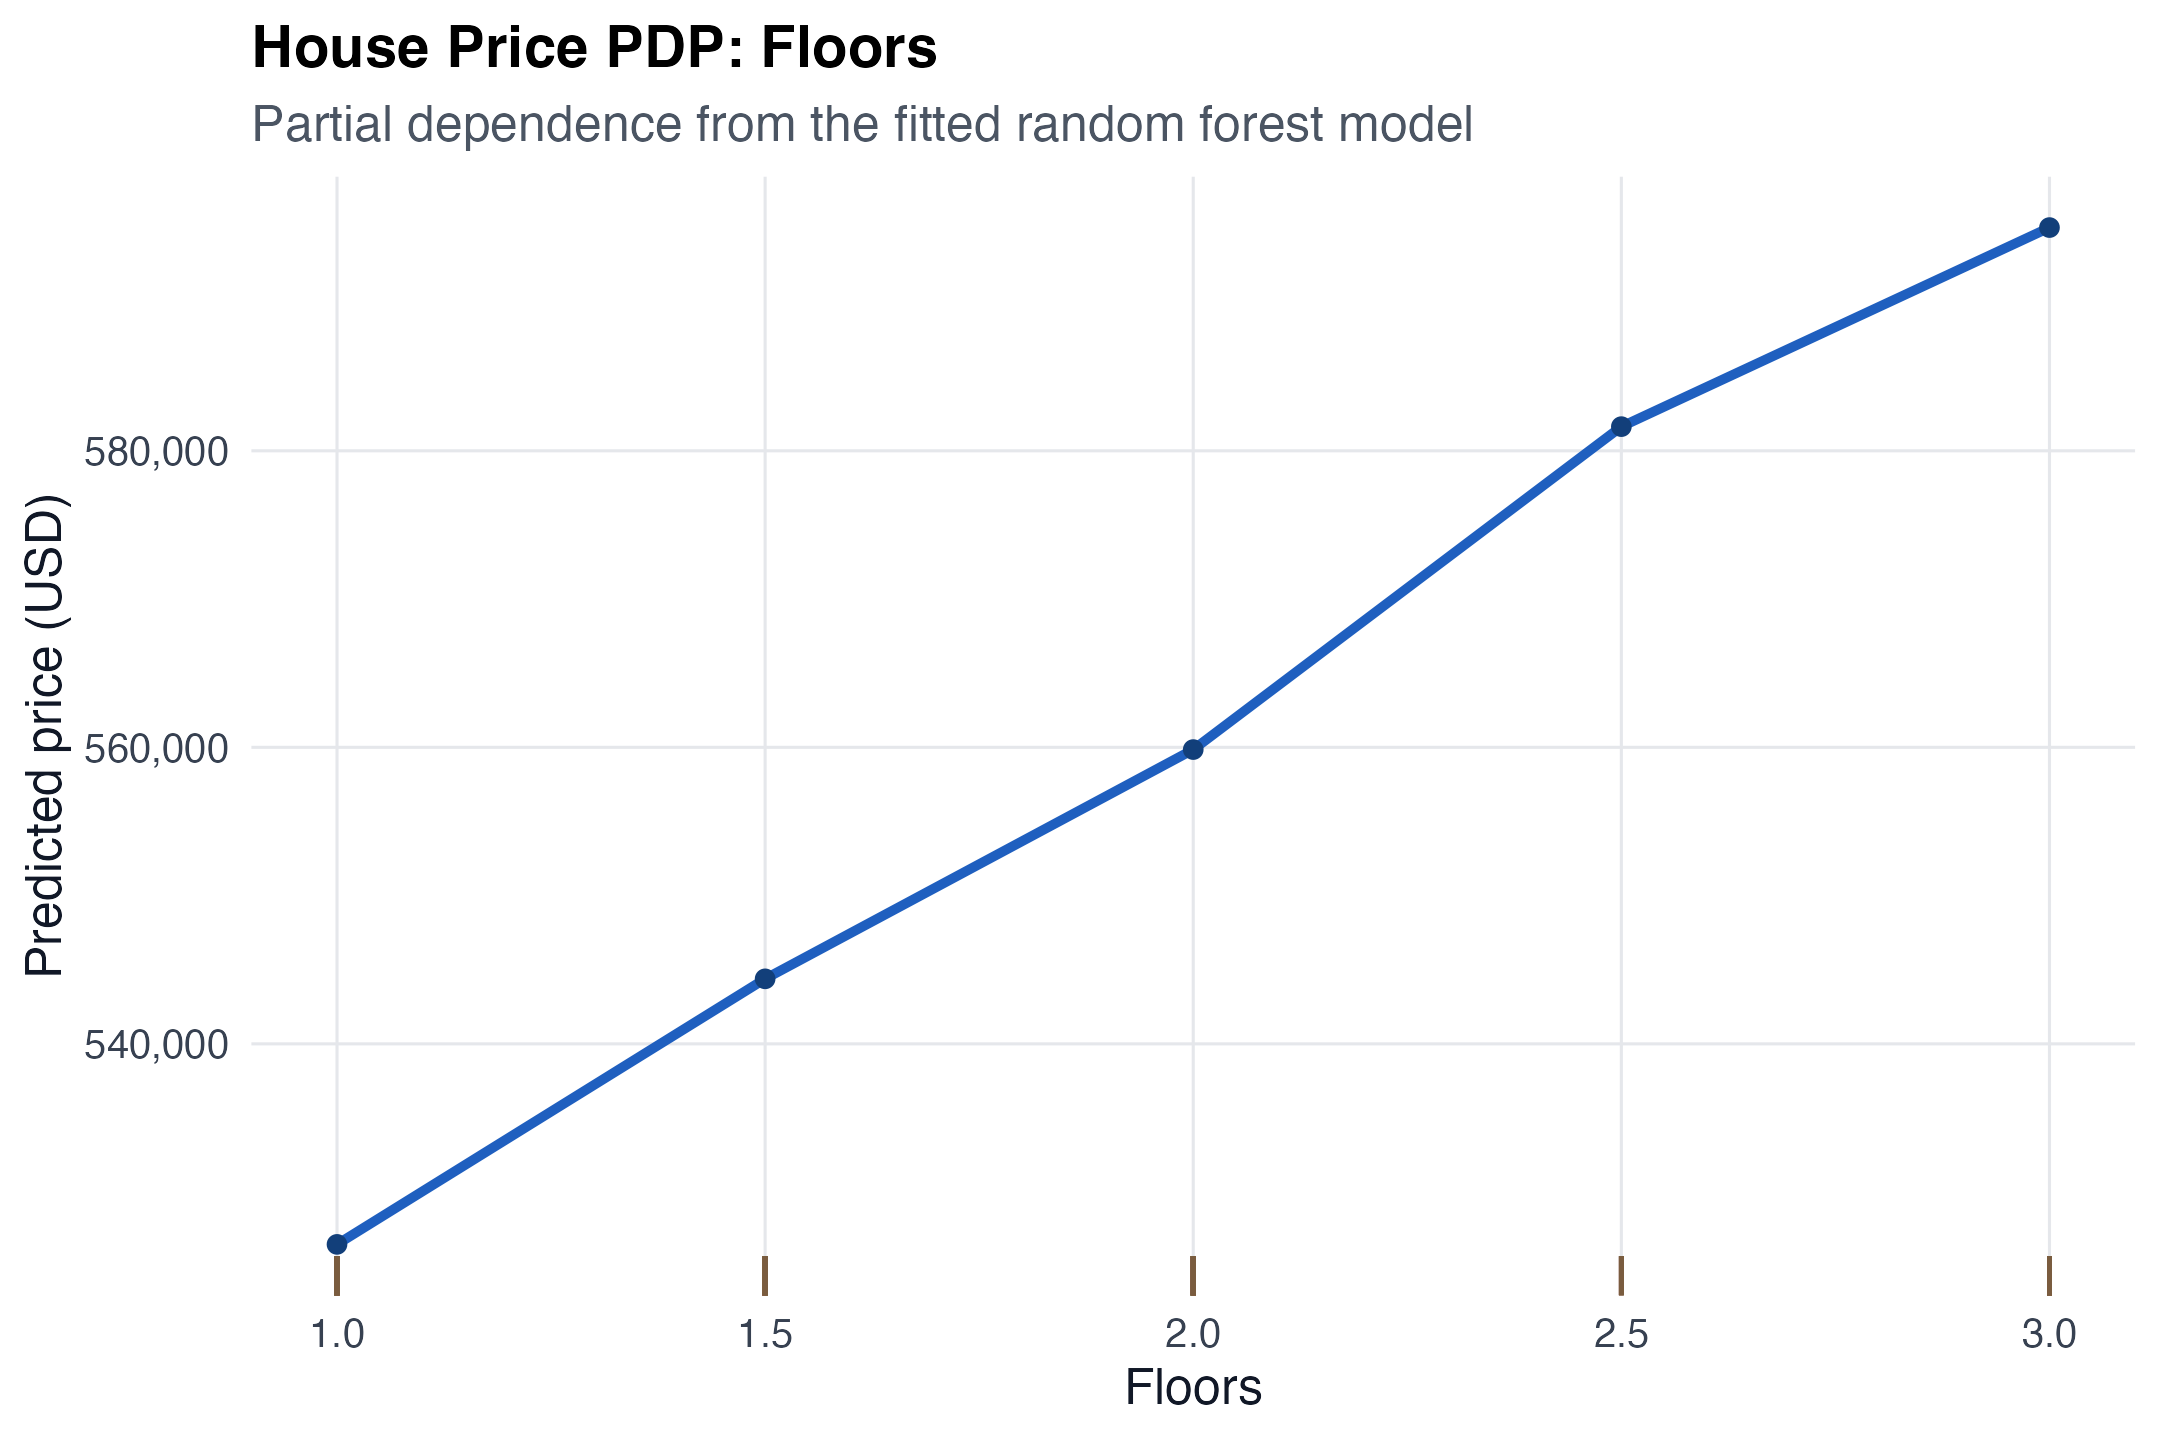
\includegraphics[width=0.46\textwidth]{house_pdp_floors.png}
\end{tabular}
\caption{One-dimensional PDPs for King County house prices using the 1500-row house sample.}
\end{figure}

\textbf{Bedrooms.}
Bedrooms have a relatively small marginal effect in this model. Predicted price changes only modestly across the observed bedroom grid compared with the effects of living area and bathrooms. For valuation work, bedroom count should not be interpreted in isolation; its value depends heavily on the size and quality characteristics represented by other variables.

\textbf{Bathrooms.}
Bathrooms show a positive relationship with predicted price. The PDP rises from about \$497,000 at the low end to about \$832,000 at the high end. In business terms, this suggests bathrooms are a meaningful property value signal, likely because they proxy for both functionality and higher-end property layouts.

\textbf{Living area.}
Living area is the clearest price driver. The PDP increases strongly from smaller homes to larger homes, with predicted price rising by more than \$800,000 across the plotted range. This is the most actionable property feature in the selected model: pricing, appraisal review, and customer segmentation should prioritize living area before interpreting room counts.

\textbf{Floors.}
Floors have a moderate positive marginal effect. Predicted price is higher for multi-floor homes, but the range is much smaller than for living area. This suggests that floors may reflect style, location, or layout preferences, but it is not the primary pricing lever in this feature set.

\section{Conclusions}

For the bike rental business, the model supports three planning rules. First, demand has a strong upward time trend in the observed period. Second,  temperature is a major demand driver, with the best predicted performance at moderate-to-warm values. Third, high humidity and high windspeed should reduce short-term demand expectations. The two-dimensional PDP adds that warm weather is most valuable when humidity is not high.

For the house price business, the model supports a space-first valuation view. Living area dominates the selected feature set, bathrooms add a meaningful premium, and bedrooms contribute much less once the other features are held in the model. This helps avoid over-weighting bedroom count in pricing decisions when the underlying square footage does not support a higher valuation.

\section{GitHub Repository Structure}

The repository is organized as follows:

\begin{itemize}
\item Code: \texttt{src/main.R}
\item Figures: \texttt{outputs/figures/}
\item Tables: \texttt{outputs/tables/}
\item Report: \texttt{report/main.tex} and \texttt{report/main.pdf}
\end{itemize}


\end{document}
